% siminos/atlas/cut.tex  pdflatex atlas
% $Author$ $Date$

\section{Poincar\'e sections}
\label{s:cut}

In the {\em Poincar\'e section method} one records the coordinates of a
trajectory $\ssp(\zeit)$ at the instant it traverses an oriented fixed
hypersurface $\PoincS$ of codimension 1, $\sspRed_n = \ssp(\zeit_n) \in
\PoincS$. For high-dimensional flows that we have in mind the only
feasible section is a hyperplane, the type of Poincar\'e section (or,
from now on, just a \emph{section})  we shall consider here. Such a
section is almost always only local, and captures important features of
the flow only in an open neighborhood of the section-fixing \template.

%%%%%%%%%%%%%%%%%%%%%%%%%%%%%%%%%%%%%%%%%%%%%%%%%%%%%%%%%%%%%%%%%%%%%
\begin{figure}
  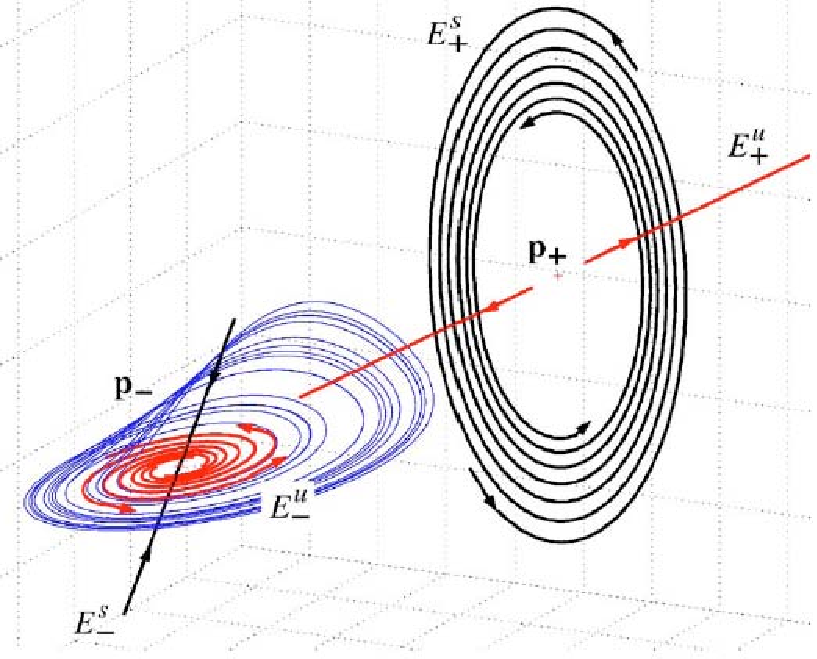
\includegraphics[width=0.3\textwidth]{AmLeAg06Im1}
    \caption{[From \refref{AmLeAg06}]
R\"ossler \eqva\ and their invariant manifolds. The stable manifold of
the inner {\eqv} $\ssp_{-}$  is 1-dimensional and the unstable one is a
spiral-out focus. For the outer {\eqv} $\ssp_{+}$  the stable manifold is
a spiral-in focus (basin boundary for initial conditions that either fall
into the chaotic attractor, or escape to infinity) and the unstable
manifold is 1-dimensional.
    }
\label{fig:AmLeAg06Im1}
\end{figure}
%%%%%%%%%%%%%%%%%%%%%%%%%%%%%%%%%%%%%%%%%%%%%%%%%%%%%%%%%%%%%%%%%%%%%

As an example consider the system of R\"ossler\rf{ross},
\index{R\"ossler system}
\beq
\begin{split}
  \dot{x} &= -x \,-\,z \\
  \dot{y} &= x + a y \\
  \dot{z} &= b + z (x - c)
  \,,
  \label{eq:Rossler}
\end{split}
\eeq
where $a = b = 0.2$ and $c = 5.7$. This flow has two prominent invariant states,
the `inner' unstable \eqv\ $\ssp_{-}$ and the `outer' $\ssp_{+}$ (Fig. \ref{fig:AmLeAg06Im1})
which we pick as {\em \template s}. A section that pass through either of these
points captures nearby trajectories whose short-time dynamics resembles that of the
\template.

We orient the sections so the section plane $\PoincS_{-}$ contains the
1\dmn\ stable eigenvector (\reffig{fig:RoessSct1}), and the other section
$\PoincS_{+}$ contains the 1\dmn\ unstable eigenvector
(\reffig{fig:RoessSct2}), thus capturing all of the local spiral-in,
spiral-out dynamics.

The remaining freedom
to rotate each section can be used to orient them in such a fashion that
the ridge
(the intersection of the two sections, indicated by the brown line in
individual sections in the figures) lies approximately midways between the
two templates (\reffig{fig:RoessSctAtlas}).
    \DB{2012-04-10}{
    Not really sure how this last bit fits into this part at this time.
    It is unclear why we are doing this. I would consider moving this to
    discussion of 2-chart atlas. 2012-04-10 Predrag: is the text better
    now?
    }

A well chosen section captures the dynamics in the neighborhood of its
\template, but far does this neighborhood extend along the hyperplane?
The answer is that the section captures neighboring trajectories as long
as it cuts them transversally; it fails the moment the velocity field at
point $\sspRSing$ fails to pierce the section. At these locations, the
velocity either vanishes (\eqv) or is tangent to the section, \ie,
orthogonal to the section normal $\hat{n}$,
\(
    \hat{n} \cdot \vel(\sspRSing) = 0
\,,\qquad
    \sspRSing \in \cal{S}
\,.
\) %ee{eq:sspRSing}
    \DB{2012-04-10}{
    Are we using $S$ or ${\cal S}$ as the variable for the
    section border? Both are used in the text.\\
    Predrag: ${\cal S}$ is more consistent with $\pS$ and $\PoincS$ notation}
For a smooth flows such points form a smooth $(d\!-\!2)$\dmn\ \emph{\poincBord} ${\cal S} \subset \PoincS$
encompassing the open neighborhood of the {\template} characterized by
qualitatively similar flow. We shall refer to such region of a section hyperplane
as a `chart' of the {\template} neighborhood.
%    \DB{2012-04-10}{
%    As of today `chart' is undefined in the text up to this point}
      \DB{2012-04-10}{As of today \reffig{fig:A29PoincBad} about good and bad Poincare
      sections went to Flotsam. Are we going to put it back or are we
      dropping it and should ``correctly'' be dropped.
      Predrag: I think we drop it, for brevity's sake}


For R\"ossler flow \refeq{eq:Rossler}
[blah blah]
%\subsection{R\"ossler two-chart atlas}

\subsection{R\"ossler unstable manifold curvilinear distance}
\subsection{R\"ossler return map}
\subsection{$N$-chart atlas, forward maps}
% \subsection{Ring of Fire return map\rf{lanCvit07}}

    \ifdraft\color{blue}


The two charts
\reffigs{fig:RoessSct1}{fig:RoessSct2} illustrate \poincBord,
and \reffigs{fig:RoessSctAtlas} the combined 2-chart atlas.

%%%%%%%%%%%%%%%%%%%%%%%%%%%%%%%%%%%%%%%%%%%%%%%%%%%%%%%%%%%%%%%%%%%%%
\begin{figure}%[H]
\begin{center}
  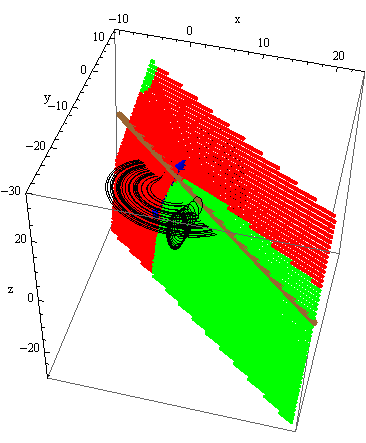
\includegraphics[width=0.30\textwidth,clip=true]{RoessSct1}
\end{center}
  \caption{\label{fig:RoessSct1}
  A R\"ossler flow Poincar\'e section $\PoincS_{-}$ centered on the inner
  {\eqv} $\ssp_{-}$ \template\ and its stable eigenvector.
}
\end{figure}
%%%%%%%%%%%%%%%%%%%%%%%%%%%%%%%%%%%%%%%%%%%%%%%%%%%%%%%%%%%%%%%%%%%%%

%%%%%%%%%%%%%%%%%%%%%%%%%%%%%%%%%%%%%%%%%%%%%%%%%%%%%%%%%%%%%%%%%%%%%
\begin{figure}%[H]
\begin{center}
  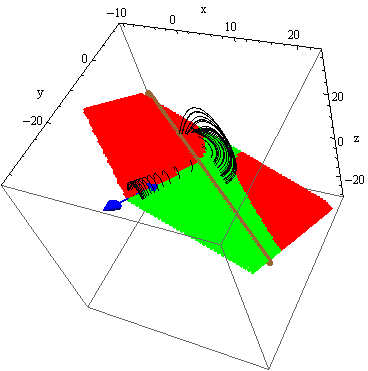
\includegraphics[width=0.30\textwidth,clip=true]{RoessSct2}
\end{center}
  \caption[R\"ossler section, outer {\eqv}]{
  A Poincar\'e section for R\"ossler flow
      centered on the
      outer
  {\eqv} $\ssp_{+}$ \template.
  } \label{fig:RoessSct2}
\end{figure}
%%%%%%%%%%%%%%%%%%%%%%%%%%%%%%%%%%%%%%%%%%%%%%%%%%%%%%%%%%%%%%%%%%%%%

%%%%%%%%%%%%%%%%%%%%%%%%%%%%%%%%%%%%%%%%%%%%%%%%%%%%%%%%%%%%%%%%%%%%%
\begin{figure}%[H]
\begin{center}
  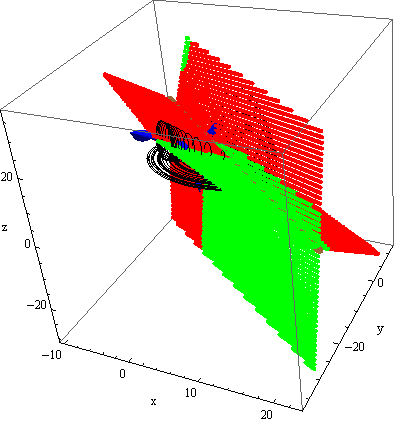
\includegraphics[width=0.30\textwidth,clip=true]{RoessSctAtlas}
\end{center}
  \caption{
  A two-section atlas for R\"ossler flow, with the local sections of
  \reffigs{fig:RoessSct1}{fig:RoessSct2} oriented and combined so the
  Euclidean distance from the first \template\ to the ridge (intersection
  of the two sections, indicated by the brown line in individual sections
  of the preceding figures), and then to the second \template\ is
  approximately minimized.
  } \label{fig:RoessSctAtlas}
\end{figure}
%%%%%%%%%%%%%%%%%%%%%%%%%%%%%%%%%%%%%%%%%%%%%%%%%%%%%%%%%%%%%%%%%%%%%

%%%%%%%%%%%%%%%%%%%%%%%%%%%%%%%%%%%%%%%%%%%%%%%%%%%%%%%%%%%%%%%%%%%%%
\begin{figure}
\begin{center}
(a) % 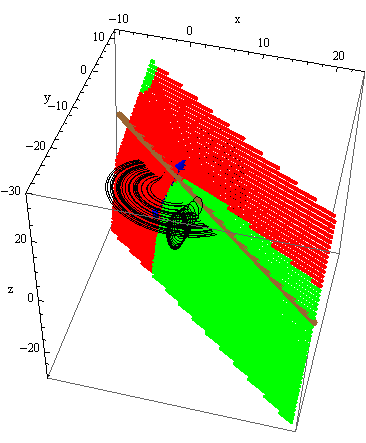
\includegraphics[width=0.30\textwidth,clip=true]{RoessSct1}
(b) 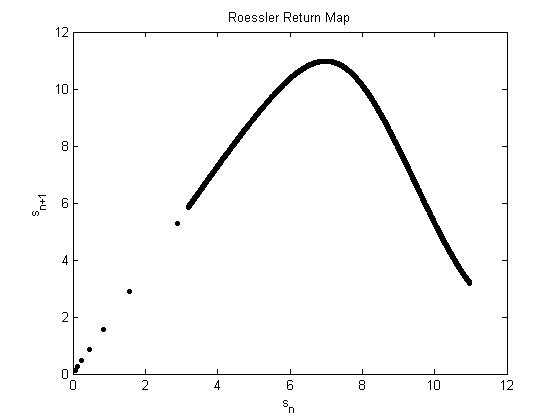
\includegraphics[width=0.30\textwidth,clip=true]{RoessRetMap}
\end{center}
  \caption{
(a) R\"ossler strange attractor section of \reffig{RoessSct1}
(b) R\"ossler return map for curvilinear distance as measured
along the unstable manifold section (the method of
\refref{Christiansen97}, see \refrefs{DasBuchBasu07}).
  }
\label{fig:RoessRetMap}
\end{figure}
%%%%%%%%%%%%%%%%%%%%%%%%%%%%%%%%%%%%%%%%%%%%%%%%%%%%%%%%%%%%%%%%%%%%%

In general there are two strategies for replacing a continuous-time flow
by iterated mappings; by cutting it by Poincar\'e sections, or by
\emph{strobing} it at a sequence of instants in time. While
`strobing' is what any numerical integrator does, by representing a
trajectory by a sequence of time-integration step separated points,
strobing is in general not a reduction of a flow, as the sequence of
strobed points still resides in the full \statesp\ $\pS$, of
dimensionality $d$.

A Poincar\'e section is {\em not} a projection onto a lower-dimensional
space: Rather, it is a local change of coordinates to a direction along
the flow, and the remaining coordinates (spanning the section) transverse
to it. No information about the flow is lost; the full space trajectory
can always be reconstructed by integration from the nearest point in the
section.


An example of a wurst is the set of group orbits traced out by a single
short \rpo\ in \reffig{fig:CLf01group}. As \cLe\ exhibits only the simplest,
$m=1$ Fourier mode, all group orbits are circles, which appear elliptical in
most $d=5 \to 3$~dimensions projections.
    \PC{define \cLe, refer to \reffig{fig:CLf01group}}
    \color{black}\fi

Any state in the  group orbit set $\pS_{\ssp}$
is physically equivalent to any other. The action of a symmetry group
thus stratifies the \statesp\ into a union of group orbits,
\reffig{fig:BeThTraj}\,{(a)}.

\subsection{\Statesp\ visualization}

On perils of thinking linearly: bases such as Fourier modes are
perfectly natural for problems such a bifurcation of a steady state, and
other weak perturbations. They are absolutely unnatural for strongly
nonlinear problems, with many Fourier modes of comparable magnitude and
strongly entangled.

\subsection{\CLe}

The \cLe\rf{GibMcCLE82} are given by
\beq
\begin{split}
  \dot{x} &= -\sigma x \,+\,\sigma y \\
  \dot{y} &= (\rho-z)\,x\,-\,a y \\
  \dot{z} &= \dfrac{1}{2}(x y^* + x^* y) - b z
  \,,
  \label{eq:ComplexLorenz}
\end{split}
\eeq
where $x$, $y$ are complex variables, $z$ is real, the parameters
$\sigma$ and $b$ are real, and the parameters $\rho = \rho_1 + i \rho_2$
and $a = 1 - i e$ are complex.

\subsection{Experimentalist description: a video 1D to 3D arrays of pixels}
\subsection{Theorist description: $\infty$-\dmn\ \statesp}
\subsection{Time orbit: point is a point, line is a line in all dimensions}
\label{sect:TimeOrb}

\subsection{Physical dimension: covariant Lyapunov vectors}
